
\documentclass[runningheads]{LaTeX2e_Proceedings_Templates/llncs}

\usepackage{graphicx}
\usepackage{booktabs}
\usepackage{array}

\begin{document}

\title{Supplementary Material for UAV-TAlign: Scene-Level RGB-Thermal Alignment for Cross-FOV UAV Imagery}
\titlerunning{Supplementary Material for UAV-TAlign}

\author{Anonymous Authors}
\authorrunning{Anonymous Authors}

\institute{Anonymous submission for PRCV 2026}

\maketitle

\section{Dataset and Scene Details}

This supplement provides additional scene statistics, diagnostic tables, ablation details, and raw
RGB/T qualitative examples. The main paper is self-contained; the material here is intended to make
protocol choices and empirical trends easier to inspect. All examples are raw paired inputs from the
released evaluation subset, not synthesized rectification visualizations.

\begin{table}[t]
\centering
\scriptsize
\setlength{\tabcolsep}{3pt}
\resizebox{\textwidth}{!}{%
\begin{tabular}{llllllllrr}
\toprule
ID & Light & Thermal & View & Scene family & Pairs & Canonical & Acc. \% & Edge gain & Grad. gain \\
\midrule
01 & day & grayscale & wide & substation power lines & 50 & Pass & 98.0 & 0.145 & 0.125 \\
02 & day & grayscale & zoom & substation power lines & 50 & Not accepted & 98.0 & 0.043 & 0.054 \\
03 & night & grayscale & wide & substation power lines & 45 & Not accepted & 82.2 & 0.172 & 0.212 \\
04 & night & grayscale & zoom & substation power lines & 45 & Pass & 80.0 & 0.077 & 0.109 \\
05 & night & pseudocolor & - & solar panels & 16 & Not accepted & 6.2 & 0.104 & 0.110 \\
06 & day & pseudocolor & - & solar panels & 16 & Pass & 81.2 & 0.170 & 0.138 \\
07 & day & grayscale & - & transmission tower & 102 & Pass & 92.2 & 0.142 & 0.201 \\
08 & night & grayscale & - & urban & 22 & Not accepted & 36.4 & 0.113 & 0.089 \\
09 & day & pseudocolor & - & building & 20 & Pass & 70.0 & 0.115 & 0.086 \\
10 & day & pseudocolor & - & factory & 24 & Not accepted & 25.0 & 0.226 & 0.168 \\
11 & night & grayscale & - & building & 25 & Not accepted & 48.0 & 0.046 & 0.061 \\
12 & day & grayscale & - & orchard & 20 & Not accepted & 75.0 & 0.059 & 0.024 \\
13 & lowlight & pseudocolor & - & road & 21 & Pass & 61.9 & 0.289 & 0.277 \\
14 & lowlight & pseudocolor & - & transmission tower & 18 & Pass & 94.4 & 0.193 & 0.122 \\
15 & lowlight & pseudocolor & - & woodland & 26 & Not accepted & 19.2 & 0.088 & 0.022 \\
\bottomrule
\end{tabular}}
\caption{Complete scene list for UAV-TAlign-1K. The canonical column reports the scene-level decision under the QA-aware criterion used in the main paper.}
\label{tab:supp_scene_list}
\end{table}


\section{Extended Baseline Results}

Table~\ref{tab:supp_pairwise_full} reports the complete pairwise baseline summary used to support
the main-paper comparison. These metrics describe per-pair usability and should be read separately
from the scene-level canonical criterion.

\begin{table}[t]
\centering
\scriptsize
\setlength{\tabcolsep}{3pt}
\resizebox{\textwidth}{!}{%
\begin{tabular}{lrrrrrrrl}
\toprule
Method & OK/Total & OK \% & H \% & Inlier & Coverage & Reproj. & Runtime s & Note \\
\midrule
SIFT + RANSAC & 457/500 & 91.4 & 91.4 & 0.240 & 0.599 & 0.260 & 4.61 &  \\
AKAZE + RANSAC & 479/500 & 95.8 & 95.8 & 0.177 & 0.646 & 0.393 & 2.37 &  \\
Kornia LoFTR outdoor & 499/500 & 99.8 & 99.8 & 0.096 & 0.919 & 1.411 & 0.55 & max dim 1600 \\
RoMa outdoor full & 500/500 & 100.0 & 100.0 & 0.400 & 0.982 & 1.672 & 1.08 &  \\
XoFTR-640 & 494/500 & 98.8 & 98.8 & 0.151 & 0.951 & 1.610 & 1.20 &  \\
raw MINIMA & 500/500 & 100.0 & 100.0 & 0.378 & 0.996 & 1.707 & 1.86 &  \\
\bottomrule
\end{tabular}}
\caption{Complete pairwise baseline summary on the 500-pair evaluation subset.}
\label{tab:supp_pairwise_full}
\end{table}

\begin{table}[t]
\centering
\scriptsize
\setlength{\tabcolsep}{3pt}
\resizebox{\textwidth}{!}{%
\begin{tabular}{llrrrrrrrr}
\toprule
Condition & Value & Scenes & Pass & Pass \% & Acc. \% & Edge & Grad. & Reject \% & Classical OK \% \\
\midrule
light condition & day & 7 & 4/7 & 57.1 & 77.1 & 0.129 & 0.114 & 15.0 & 88.2 \\
light condition & lowlight & 3 & 2/3 & 66.7 & 58.5 & 0.190 & 0.140 & 17.7 & 87.9 \\
light condition & night & 5 & 1/5 & 20.0 & 50.6 & 0.102 & 0.116 & 19.8 & 95.8 \\
thermal rendering & grayscale & 8 & 3/8 & 37.5 & 76.2 & 0.100 & 0.109 & 19.7 & 99.1 \\
thermal rendering & pseudocolor & 7 & 4/7 & 57.1 & 51.2 & 0.169 & 0.132 & 14.2 & 81.1 \\
view & None & 11 & 5/11 & 45.5 & 55.4 & 0.140 & 0.118 & 15.4 & 87.9 \\
view & wide & 2 & 1/2 & 50.0 & 90.1 & 0.159 & 0.168 & 20.3 & 98.9 \\
view & zoom & 2 & 1/2 & 50.0 & 89.0 & 0.060 & 0.081 & 23.6 & 98.0 \\
\bottomrule
\end{tabular}}
\caption{Condition-level scene summary for the UAV-TAlign full pipeline.}
\label{tab:supp_condition_full}
\end{table}


\section{Additional Reliability Diagnostics}

The following tables expand the protocol-consistency analysis from the main paper. They are meant as
additional reliability diagnostics for the canonical scene-level criterion, not as a replacement for
manual geometric annotations.

\begin{table}[t]
\centering
\scriptsize
\setlength{\tabcolsep}{3pt}
\resizebox{\textwidth}{!}{%
\begin{tabular}{lrrrrrrrr}
\toprule
Group & Scenes & Acc. \% & Edge & Grad. & Grad improved \% & Reject \% & Severe outlier \% & Mean inlier \\
\midrule
Pass & 7 & 82.5 & 0.162 & 0.151 & 96.4 & 14.4 & 0.0 & 0.446 \\
Not accepted & 8 & 48.8 & 0.106 & 0.092 & 76.0 & 19.5 & 12.5 & 0.403 \\
\bottomrule
\end{tabular}}
\caption{Pass/not-accepted grouping under the canonical scene-level criterion.}
\label{tab:supp_passfail_proxy}
\end{table}

\begin{table}[t]
\centering
\scriptsize
\setlength{\tabcolsep}{3pt}
\resizebox{\textwidth}{!}{%
\begin{tabular}{lrrrr}
\toprule
Rule & Not-accepted true & Pass true & Not-accepted recall \% & Pass exclusion \% \\
\midrule
Baseline-relative QA outliers & 8 & 0 & 100.0 & 100.0 \\
Accepted ratio < 0.60 & 5 & 0 & 62.5 & 100.0 \\
Low accepted-ratio warning & 6 & 2 & 75.0 & 71.4 \\
Outlier signal OR accepted ratio < 0.60 & 8 & 0 & 100.0 & 100.0 \\
Outlier signal AND warning-path not OK & 8 & 0 & 100.0 & 100.0 \\
\bottomrule
\end{tabular}}
\caption{Selected reliability rules that separate conservative scene decisions from accepted scenes.}
\label{tab:supp_reliability_rules}
\end{table}

\begin{table}[t]
\centering
\scriptsize
\setlength{\tabcolsep}{3pt}
\resizebox{\textwidth}{!}{%
\begin{tabular}{llrrrrl}
\toprule
Scene & Canonical & Acc. \% & Reject \% & Edge & Grad. & QA outlier signal \\
\midrule
01 & Pass & 98.0 & 0.0 & 0.145 & 0.125 & No \\
02 & Not accepted & 98.0 & 30.6 & 0.043 & 0.054 & Yes \\
03 & Not accepted & 82.2 & 40.5 & 0.172 & 0.212 & Yes \\
04 & Pass & 80.0 & 16.7 & 0.077 & 0.109 & No \\
\bottomrule
\end{tabular}}
\caption{Paired-control scenes used to inspect whether the reliability criterion captures scene-level behavior beyond pairwise match availability.}
\label{tab:supp_paired_controls}
\end{table}


\section{Cumulative Ablations and Random-Selection Sensitivity}

The cumulative ablation is reported on a fixed 8-scene subset and is used to separate candidate
selection, robust aggregation, and QA-aware scene decision. The random-selection supplement keeps the
same subset and changes only the random seed, showing why deterministic-even selection is used as a
stable default operating policy.

\begin{table}[t]
\centering
\scriptsize
\setlength{\tabcolsep}{3pt}
\resizebox{\textwidth}{!}{%
\begin{tabular}{llllrrrrrr}
\toprule
Stage & Candidate & Aggregation & Decision & Pass & Acc. \% & Edge & Grad. & Reject \% & Severe \% \\
\midrule
A1 & forced adaptive & single best & accepted only & 8/8 & 77.4 & 0.124 & 0.126 & 18.1 & 10.4 \\
A2 & forced adaptive & robust weighted & accepted only & 8/8 & 77.4 & 0.145 & 0.148 & 18.1 & 4.2 \\
A3 & forced adaptive & robust weighted & qa status & 5/8 & 77.2 & 0.147 & 0.149 & 19.0 & 4.2 \\
S1 & forced adaptive random & robust weighted & qa status & 6/8 & 80.9 & 0.158 & 0.169 & 19.4 & 3.1 \\
A4-subset & formal default slice & robust weighted & qa status & 5/8 & 80.4 & 0.147 & 0.149 & 20.9 & 4.2 \\
A4-all & formal default & robust weighted & qa status & 7/15 & 64.5 & 0.132 & 0.120 & 17.1 & 6.7 \\
\bottomrule
\end{tabular}}
\caption{Cumulative ablation summary and the formal-run slice on the same 8-scene subset.}
\label{tab:supp_ablation_full}
\end{table}

\begin{table}[t]
\centering
\scriptsize
\setlength{\tabcolsep}{3pt}
\resizebox{\textwidth}{!}{%
\begin{tabular}{lrrrl}
\toprule
Seed & Pass & Scenes & Pass \% & Note \\
\midrule
seed0 & 6 & 8 & 75.0 & Original single-seed S1 run. \\
seed1 & 4 & 8 & 50.0 & Random-selection supplement. \\
seed2 & 7 & 8 & 87.5 & Random-selection supplement. \\
seed3 & 5 & 8 & 62.5 & Random-selection supplement. \\
range\_across\_seed0\_to\_seed3 & 4-7 & 8 & 50.0-87.5 & Seed-sensitive spread on the same fixed subset. \\
\bottomrule
\end{tabular}}
\caption{Random-selection multi-seed summary on the fixed 8-scene ablation subset.}
\label{tab:supp_s1_seed_summary}
\end{table}

\begin{table}[t]
\centering
\scriptsize
\setlength{\tabcolsep}{3pt}
\resizebox{\textwidth}{!}{%
\begin{tabular}{llllllr}
\toprule
Scene & A3 & Seed0 & Seed1 & Seed2 & Seed3 & Random pass count \\
\midrule
01 & Pass & Not accepted & Not accepted & Pass & Not accepted & 1 \\
02 & Not accepted & Not accepted & Not accepted & Not accepted & Not accepted & 0 \\
03 & Not accepted & Pass & Not accepted & Pass & Not accepted & 2 \\
04 & Pass & Pass & Pass & Pass & Pass & 4 \\
07 & Pass & Pass & Pass & Pass & Pass & 4 \\
08 & Not accepted & Pass & Not accepted & Pass & Pass & 3 \\
13 & Pass & Pass & Pass & Pass & Pass & 4 \\
14 & Pass & Pass & Pass & Pass & Pass & 4 \\
\bottomrule
\end{tabular}}
\caption{Scene-level stability for deterministic A3 and random-selection seeds.}
\label{tab:supp_s1_scene_stability}
\end{table}


\section{Additional Qualitative Examples}

Figure~\ref{fig:supp_paired_controls} shows raw paired controls from the substation scene family.
Figure~\ref{fig:supp_representative_examples} shows additional cross-condition examples used to
inspect the range of scene appearance. These figures intentionally show raw RGB/T inputs only; no
post-hoc rectification visualizations are introduced in the supplement.

\begin{figure}[t]
\centering
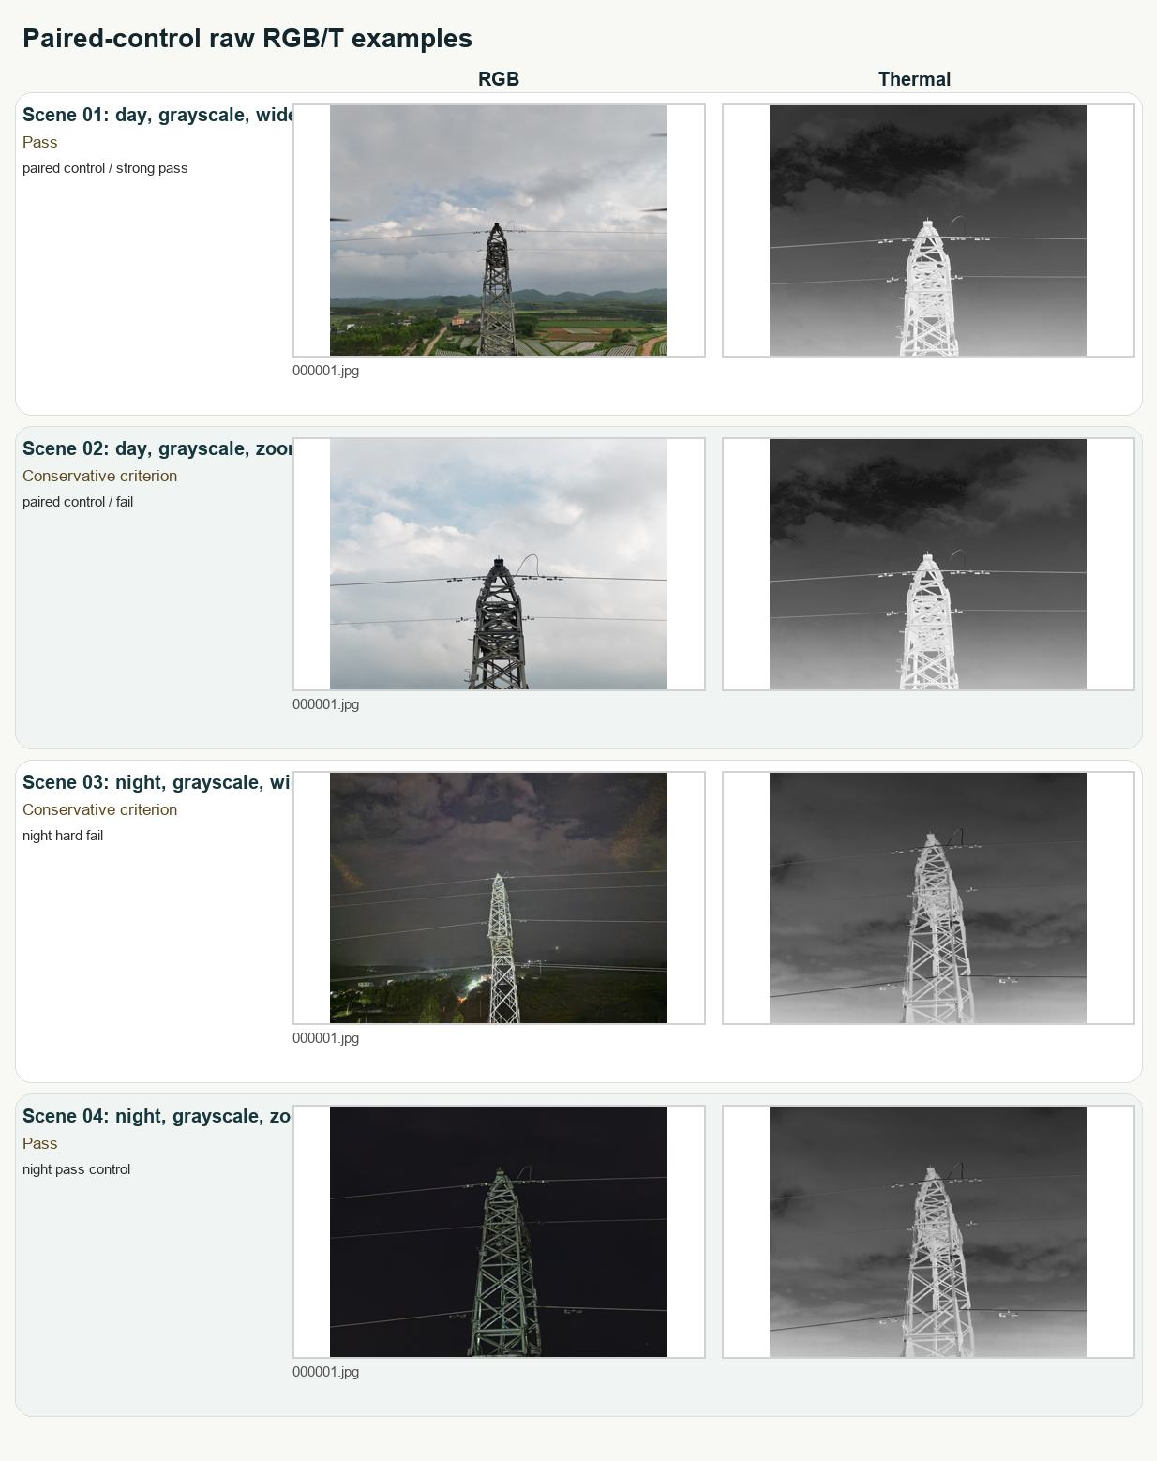
\includegraphics[width=\textwidth]{supplement_figures/supp_raw_paired_controls.pdf}
\caption{Raw RGB/T paired-control examples. Scenes 01/02 share the day substation family under
wide/zoom views, while scenes 03/04 provide a night counterpart.}
\label{fig:supp_paired_controls}
\end{figure}

\begin{figure}[t]
\centering
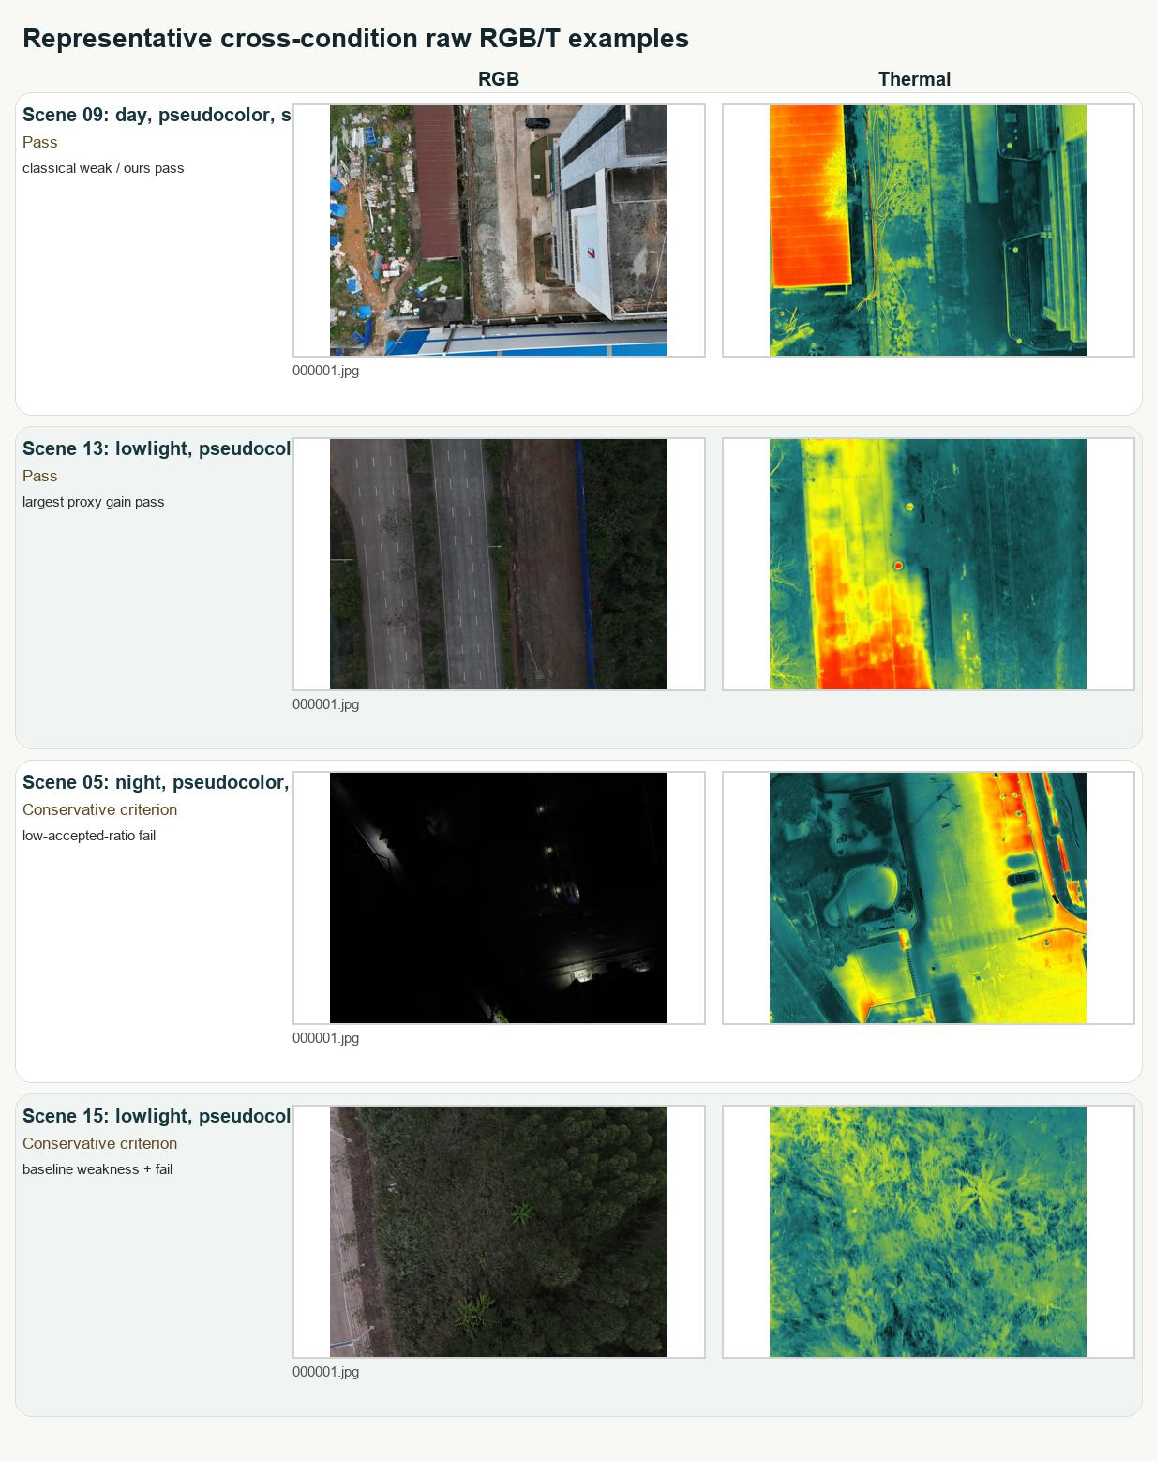
\includegraphics[width=\textwidth]{supplement_figures/supp_raw_representative_examples.pdf}
\caption{Additional raw RGB/T examples spanning pseudocolor, low-light, and challenging scene
conditions. These examples complement the main-paper dataset figure without adding synthetic or
unverified alignment visualizations.}
\label{fig:supp_representative_examples}
\end{figure}

\end{document}
